% 2007 年全国大纲卷Ⅰ理科第 7 题：正四棱柱
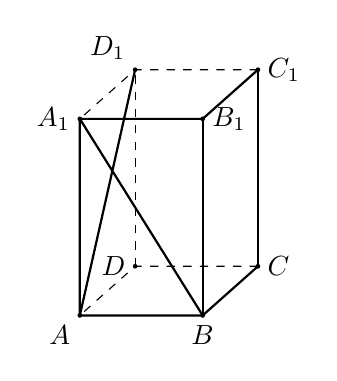
\begin{tikzpicture}[>=stealth,scale=0.78]
  \coordinate (A) at (0,0); \coordinate (B) at (2.0,0);
  \coordinate (C) at (2.9,0.8); \coordinate (D) at (0.9,0.8);
  \coordinate (A1) at (0,3.2); \coordinate (B1) at (2,3.2);
  \coordinate (C1) at (2.9,4.0); \coordinate (D1) at (0.9,4.0);
  \draw[thick] (A)--(B)--(C); \draw[dashed] (C)--(D)--(A);
  \draw[thick] (A)--(A1)--(B1)--(C1);
  \draw[dashed] (C1)--(D1)--(A1);
  \draw[thick] (B)--(B1) (C)--(C1);
  \draw[dashed] (D)--(D1);
  \draw[thick] (A1)--(B) (A)--(D1);
  \fill (A) circle (1.1pt) node[below left] {$A$};
  \fill (B) circle (1.1pt) node[below] {$B$};
  \fill (C) circle (1.1pt) node[right] {$C$};
  \fill (D) circle (1.1pt) node[left] {$D$};
  \fill (A1) circle (1.1pt) node[left] {$A_1$};
  \fill (B1) circle (1.1pt) node[right] {$B_1$};
  \fill (C1) circle (1.1pt) node[right] {$C_1$};
  \fill (D1) circle (1.1pt) node[above left] {$D_1$};
\end{tikzpicture}
